\chapter{基于输入扰动的改进}


\section{引言}
基于输入扰动的改进

\section{梯度空间的分析}
梯度空间的分析,统计关于输入/特征图的梯度响应图

\begin{figure}[H]
    \centering
    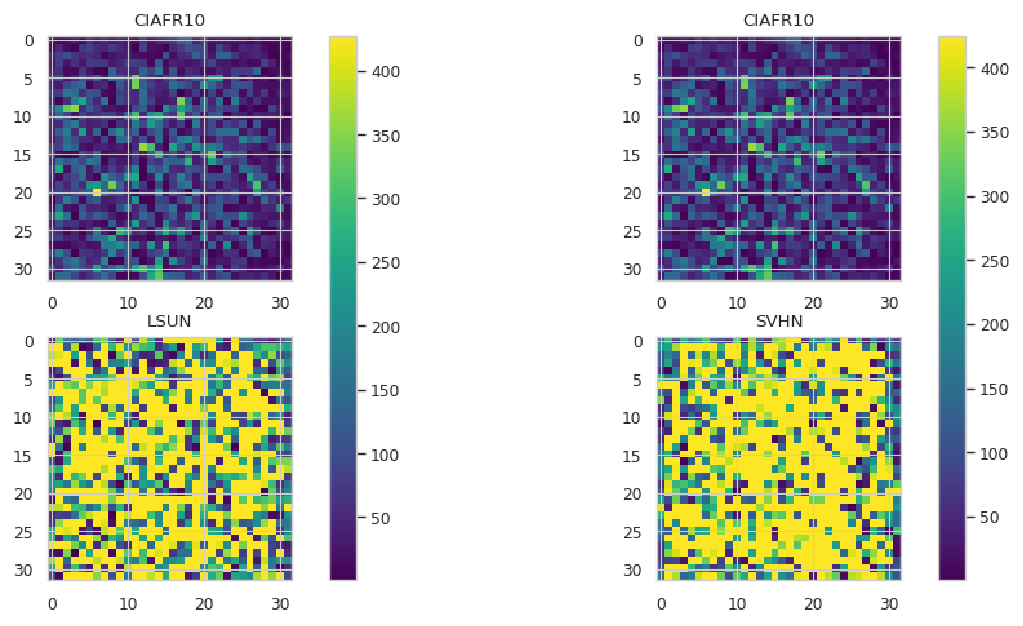
\includegraphics[width=0.75\linewidth]{assets/3-1.png}
    \caption{ResNet50 ,训练集 CIFAR10 vs OOD数据集SVHN
}
    \label{fig:enter-label}
\end{figure}

\begin{figure}[H]
    \centering
    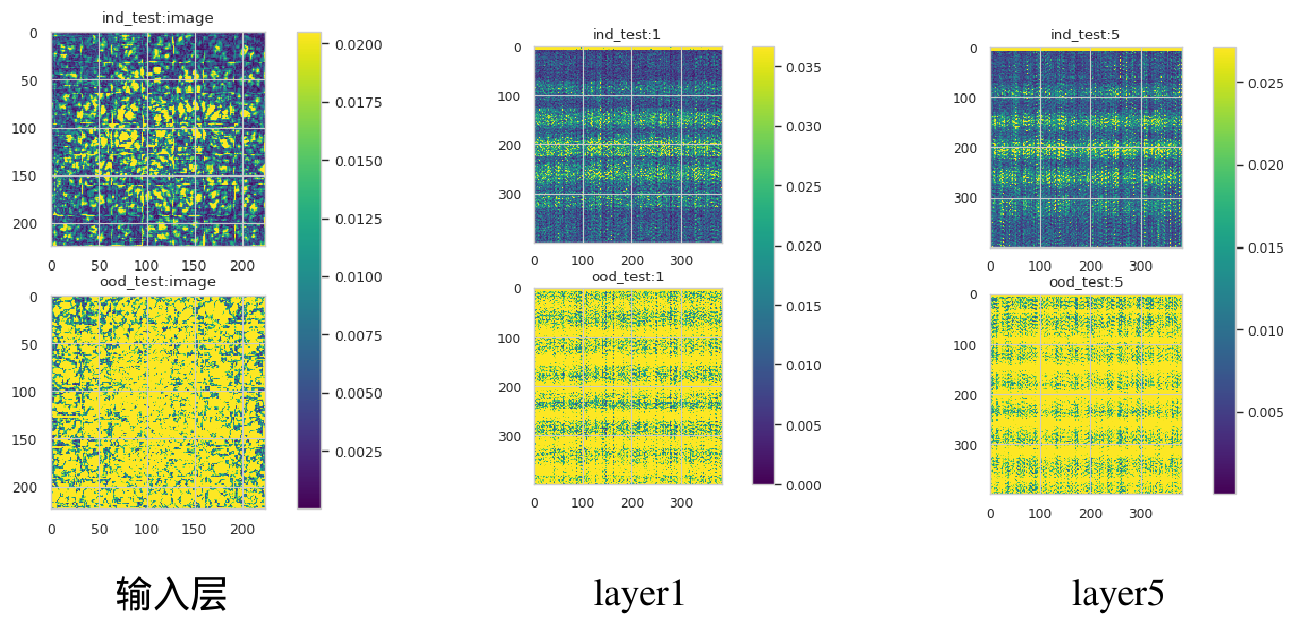
\includegraphics[width=0.75\linewidth]{assets/3-2.png}
    \caption{VIT,训练集 CIFAR10 vs OOD数据集SVHN
}
    \label{fig:enter-label}
\end{figure}

\subsection{GradNorm的分析}
直接使用gardNorm作为不确定性的度量
\begin{table}[H]
	\centering
	\resizebox{\linewidth}{!}{
		\begin{tabular}{ |P{3cm}|P{3cm}|P{3cm}|  }
			\hline
			OOD dataset& auroc($\uparrow$) & auprc ($\uparrow$) \\
			\hline
			svhn & 0.9480 & \textbf{0.9613} \\
			lsun &   \textbf{0.9287} & \textbf{0.9444} \\
			cifar100 & \textbf{0.9058} & \textbf{0.9242} \\
			mnist   & \textbf{0.9665 }&\textbf{ 0.9770} \\
			\hline
			
			svhn+ip&\textbf{ 0.9493} & 0.9599\\
			lsun+ip &  0.8990 & 0.9137 \\
			cifar100+ip& 0.8871 & 0.9027\\
			mnist+ip  &  0.9481 & 0.9550\\
			\hline
		\end{tabular}
	}
	\caption{
		resnet50+cafar10,accuracy=0.9489,gradNorm
	}
\end{table}


\begin{table}[H]
	\centering
	\resizebox{\linewidth}{!}{	
		\begin{tabular}{ |P{3cm}|P{3cm}|P{3cm}|  }
			\hline
			OOD dataset& auroc($\uparrow$) & auprc ($\uparrow$) \\
			\hline
			svhn & 0.9293 & 0.9516 \\
			lsun &   \textbf{0.9436} & \textbf{0.9563} \\
			cifar100 & \textbf{0.9426} & \textbf{0.9480} \\
			mnist   & \textbf{0.9550 }&\textbf{ 0.9680} \\
			\hline
			
			svhn+ip&\textbf{ 0.9467} &\textbf{ 0.9633}\\
			lsun+ip &  0.9175 & 0.9469 \\
			cifar100+ip& 0.9086 & 0.9317\\
			mnist+ip  &  0.9113 & 0.9286\\
			\hline
		\end{tabular}
	}
	\caption{
		vit+cafar10,accuracy=0.9600,gradNorm
	}
\end{table}


\section{输入扰动}
加入输入扰动
加入输入扰动,对比Uncertainty的分布
\begin{figure}[H]
    \centering
    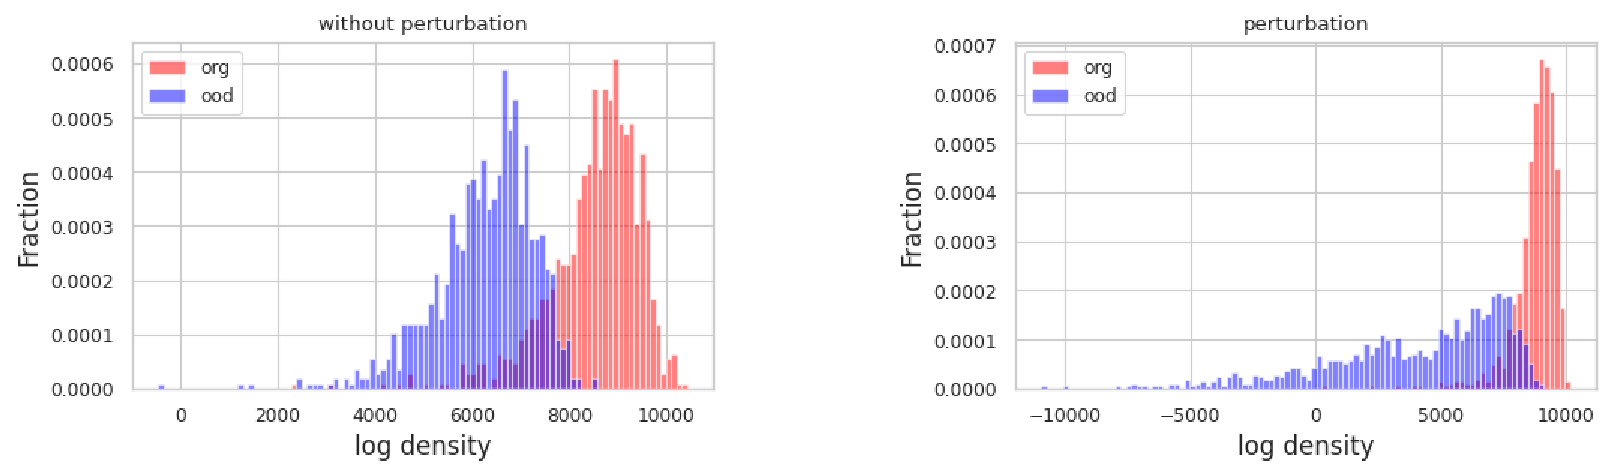
\includegraphics[width=0.75\linewidth]{assets/3-3.png}
    \caption{ResNet50 ,训练集 CIFAR10 vs OOD数据集SVHN}
    \label{fig:enter-label}
\end{figure}
\begin{figure}[H]
    \centering
    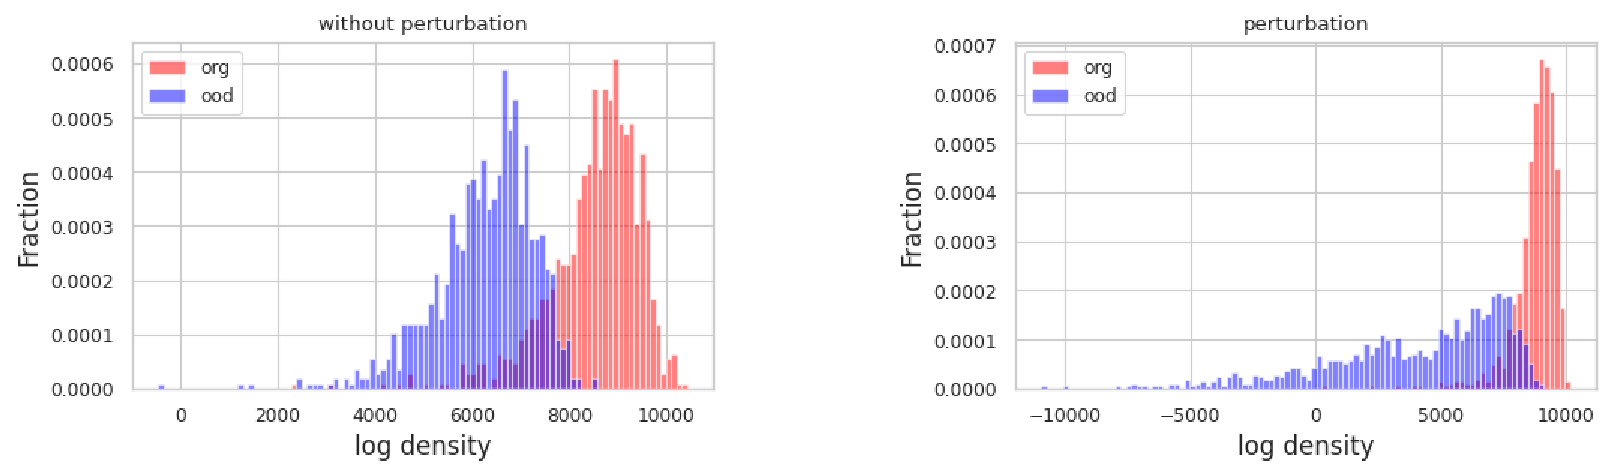
\includegraphics[width=0.75\linewidth]{assets/3-4.png}
    \caption{VIT ,训练集 CIFAR10 vs OOD数据集SVHN}
    \label{fig:enter-label}
\end{figure}

\subsection{算法流程图}
\begin{algorithm}[H]
	\caption{基于输入扰动的概率密度建模的模型不确定性算法}
	\label{alg:1}
	
	\begin{algorithmic}[1]
		\Require 训练集: $(X,Y)$ 
		\Require 谱归一化的高维特征提取网络: $f_{\theta}:x \rightarrow \mathbf{R}^d $ 
		\Require GMM模型: $q(z) = \sum_{y}q(z|y=c)q(y=c)$
		
		\\
		\Procedure {1.训练阶段}{}
		\State 在训练数据集数据集上训练网络$f_{\theta}$
		\For {属于类别c的样本}
		\State $\mu_{c}=\frac{1}{|x_c|}f_{\theta}(x_c)$
		\State $\Sigma_c = \frac{1}{|x_c|-1}(f_{\theta}(x_c)-\mu_c)(f_{\theta}(x_c)-\mu_c)^T$
		\State q(y=c)=$\frac{|X_C|}{|X|}$
		\EndFor
		\EndProcedure

		
		\\
		\Procedure {2.模型不确定性计算}{}
		\State $z=f_{\theta}(x)$
		\State  $q(z) = \sum_{y}q(z|y=c)q(y=c)$,其中$q(z)\sim N(\mu_c,\Sigma_c)$
		\State $\tilde{x}=x+\epsilon* \cdot sign(\nabla_x \log q(z)))$,其中$\epsilon$通过grid search调参
		\State $\tilde{z}=f_{\theta}(\tilde{x})$
		\State 计算模型不确定性 $Uncertainty(x) = \sum_{y}q(\tilde{z}|y=c)q(y=c)$,其中$q(\tilde{z})\sim N(\mu_c,\Sigma_c)$
		\EndProcedure
	\end{algorithmic}
\end{algorithm}



\section{实验结果与分析}
在OOD检测任务上,对抗样本检测任务上,主动学习任务上评估。
\subsection{OOD检测任务上评估}



\subsubsection{Cifar加入输入扰动前后对比}
\begin{table}[H]
	\centering
	\resizebox{\linewidth}{!}{
		
		\begin{tabular}{ |P{3cm}|P{3cm}|P{3cm}|  }
			\hline
			OOD dataset& auroc($\uparrow$)  & auprc($\uparrow$)  \\
			\hline
			svhn & \textbf{0.9221} & \textbf{0.9432} \\
			lsun &   0.9363 & 0.9528 \\
			cifar100 & 0.8861 & \textbf{0.9028} \\
			mnist   & 0.9189 & 0.9369 \\
			tiny-imagenet & 0.9318 & 0.9479 \\
			\hline
			
			svhn+ip& 0.9216 & 0.9411\\
			lsun+ip & \textbf{ 0.9394} & \textbf{0.9533} \\
			cifar100+ip& \textbf{ 0.8885} & 0.9009\\
			mnist+ip  &  \textbf{0.9637} & \textbf{0.9666}\\
			tiny-imagenet+ip& \textbf{ 0.9397} & \textbf{0.9493}\\
			\hline
		\end{tabular}
	}
	\caption{
		vgg16+cafar10,accuracy=0.9405
	}
\end{table}



\begin{table}[H]
	\centering
	\resizebox{\linewidth}{!}{
		
		\begin{tabular}{ |P{3cm}|P{3cm}|P{3cm}|  }
			\hline
			OOD dataset& auroc($\uparrow$) & auprc ($\uparrow$) \\
			\hline
			svhn & 0.9480 & 0.9613 \\
			lsun &   0.9365 & 0.9497 \\
			cifar100 & 0.9068 & 0.9257 \\
			mnist   & 0.9774 & 0.9845 \\
			tiny-imagenet & 0.9469 & 0.9580 \\
			\hline
			
			svhn+ip&\textbf{ 0.9735} & \textbf{0.9769}\\
			lsun+ip & \textbf{ 0.9671} & \textbf{0.9716} \\
			cifar100+ip& \textbf{ 0.9171} & \textbf{0.9372}\\
			mnist+ip  &  \textbf{0.9939} & \textbf{0.9957}\\
			tiny-imagenet+ip& \textbf{ 0.9676} & \textbf{0.9731}\\
			\hline
		\end{tabular}
	}
	\caption{
		resnet50+cafar10,D=2048,accuracy=0.9489
	}
\end{table}

\begin{table}[H]
	\centering
	\resizebox{\linewidth}{!}{
		
		\begin{tabular}{ |P{3cm}|P{3cm}|P{3cm}|  }
			\hline
			OOD dataset& auroc($\uparrow$)  & auprc($\uparrow$)  \\
			\hline
			svhn & 0.9685 & 0.9768 \\
			lsun &   0.9720 & 0.9788 \\
			cifar100 & 0.9400 & 0.9514 \\
			mnist   & 0.9906 & 0.9929 \\
			tiny-imagenet & 0.9747 & 0.9803 \\
			\hline
			
			svhn+ip& \textbf{0.9891} & \textbf{0.9904}\\
			lsun+ip & \textbf{ 0.9811} & \textbf{0.9830} \\
			cifar100+ip& \textbf{ 0.9497} & \textbf{0.9585}\\
			mnist+ip  &  \textbf{0.9978} & \textbf{0.9982}\\
			tiny-imagenet+ip& \textbf{ 0.9836} & \textbf{0.9861}\\
			\hline
		\end{tabular}
	}
	\caption{
		wideResnet+cafar10,accuracy=0.9650
	}
\end{table}


\begin{table}[H]
	\centering
	\resizebox{\linewidth}{!}{
		
		\begin{tabular}{ |P{3cm}|P{3cm}|P{3cm}|  }
			\hline
			OOD dataset& auroc($\uparrow$)  & auprc($\uparrow$)  \\
			\hline
			svhn & 0.9293 & 0.9516 \\
			lsun &   0.9436 & 0.9563 \\
			cifar100 & 0.9426 & 0.9480 \\
			mnist   & 0.9550 & 0.9680 \\
			tiny-imagenet & 0.9330 & 0.9367 \\
			\hline
			
			svhn+ip& \textbf{0.9728} & \textbf{0.9793}\\
			lsun+ip & \textbf{ 0.9688} & \textbf{0.9740} \\
			cifar100+ip& \textbf{ 0.9463} & \textbf{0.9495}\\
			mnist+ip  &  \textbf{0.9904} & \textbf{0.9926}\\
			tiny-imagenet+ip& \textbf{ 0.9546} & \textbf{0.9545}\\
			\hline
		\end{tabular}
	}
	\caption{
		vit+cafar10,accuracy=0.9600
	}
\end{table}


\subsubsection{mnist加入输入扰动前后对比}
\begin{table}[H]
	\centering
	\resizebox{\linewidth}{!}{	
		\begin{tabular}{ |P{3cm}|P{3cm}|P{3cm}|  }
			\hline
			OOD dataset& auroc($\uparrow$)  & auprc($\uparrow$)  \\
			\hline
			cifar10 & 0.9949 & 0.9964 \\
			fashionmnist &   0.9914 & 0.9933 \\
			fer2013 & 0.9952 & 0.9969 \\
			lsun   & 0.9946 & 0.9962 \\
			cifar100 & 0.9945 & 0.9961 \\
			svhn & 0.9941 & 0.9960 \\
			\hline
			
			cifar10+ip&\textbf{ 0.9965} &\textbf{ 0.9974}\\
			fashionmnist+ip & \textbf{ 0.9921} & \textbf{0.9936} \\
			fer2013+ip& \textbf{ 0.9970} & \textbf{0.9978}\\
			svhn+ip  &  \textbf{0.9963} & \textbf{0.9972}\\
			cifar10+ip& \textbf{ 0.9961} & \textbf{0.9970}\\
			svhn+ip & 0.9964 & 0.9973 \\
			\hline
		\end{tabular}
	}
	\caption{
		vgg16+mnist,accuracy=0.9882
	}
\end{table}


\begin{table}[H]
	\centering
	\resizebox{\linewidth}{!}{
		\begin{tabular}{ |P{3cm}|P{3cm}|P{3cm}|  }
			\hline
			OOD dataset& auroc($\uparrow$)  & auprc($\uparrow$)  \\
			\hline
			cifar10 & 0.9949 & 0.9964 \\
			fashionmnist &   0.9914 & 0.9933 \\
			fer2013 & 0.9952 & 0.9969 \\
			lsun   & 0.9946 & 0.9962 \\
			cifar100 & 0.9945 & 0.9961 \\
			svhn & 0.9941 & 0.9960 \\
			\hline
			
			cifar10+ip&\textbf{ 0.9965} &\textbf{ 0.9974}\\
			fashionmnist+ip & \textbf{ 0.9921} & \textbf{0.9936} \\
			fer2013+ip& \textbf{ 0.9970} & \textbf{0.9978}\\
			svhn+ip  &  \textbf{0.9963} & \textbf{0.9972}\\
			cifar10+ip& \textbf{ 0.9961} & \textbf{0.9970}\\
			svhn+ip & 0.9964 & 0.9973 \\
			\hline
		\end{tabular}
	}
	\caption{
		resnet50+mnist,accuracy=0.9870
	}
\end{table}

\subsubsection{各种方法的对比}
\begin{table}[H]
		\captionsetup{labelformat=empty}
	\centering
	\resizebox{\linewidth}{!}{
\begin{tabular}{|c|c|c|c|}
\hline
Method & OOD Dataset &  AUROC($\uparrow$) & AUROC($\uparrow$) \\
\hline
\multirow{3}{*}{baseline} 
& cifar100 & 0.8786 & 0.8774 \\
& lsun & 0.8952 & 0.8997 \\
& mnist & 0.9434 & 0.9524 \\
& svhn & 0.9271 & 0.9405 \\
\hline
\multirow{3}{*}{ensemble} 
& cifar100 & 0.9244 & 0.9166 \\
& lsun & 0.9724 & 0.9685 \\
& mnist & 0.9735 & 0.9706 \\
& svhn & 0.9667 & 0.9599 \\
\hline
\multirow{3}{*}{ddu}
& cifar100 & 0.9068 & 0.9257 \\
& lsun & 0.9365 & 0.9497 \\
& mnist & 0.9774 & 0.9845 \\
& svhn & 0.9480 & 0.9613 \\
\hline
\multirow{3}{*}{ddu+ip} 
& cifar100 & 0.9171 & 0.9312 \\
& lsun & 0.9671 & 0.9716 \\
& mnist & 0.9939 & 0.9957 \\
& svhn & 0.9735 & 0.9769 \\
\hline
\end{tabular}
}
	\caption{
	resnet50+cafar10,D=2048,accuracy=0.9540
}
\end{table}

\subsubsection{GMM vs KDE 实验结果}
\begin{table}[H]
	\centering
	\resizebox{\linewidth}{!}{
		\begin{tabular}{|P{3cm}|P{3cm}|P{3cm}|}
			\hline
			OOD dataset& auroc($\uparrow$)  & auprc($\uparrow$)  \\
			\hline
			svhn+gmm & \textbf{0.9458} & \textbf{0.9564} \\
			lsun+gmm &   \textbf{0.9287} & \textbf{0.9444} \\
			cifar100+gmm & \textbf{ 0.9058 }& \textbf{0.9242} \\
			mnist +gmm  & \textbf{0.9665} & \textbf{0.9770} \\
			tiny-imagenet+gmm & \textbf{0.8932} & \textbf{0.9112} \\
			\hline
			
			svhn+kde& 0.7924 & 0.8365\\
			lsun+kde &  0.7894 & 0.8264 \\
			cifar100+kde& 0.7772 & 0.8097\\
			mnist+kde  &  0.8364 & 0.8684 \\
			tiny-imagenet+kde& 0.7653 & 0.7950\\
			\hline
		\end{tabular}
	}
	\caption{
		resnet50+cafar10,GMM vs KDE ,Dimension=2048,accuracy=0.9489
	}
\end{table}


\begin{table}[H]
	\centering
	\resizebox{\linewidth}{!}{
		
		\begin{tabular}{ |P{3cm}|P{3cm}|P{3cm}|  }
			\hline
			OOD dataset& auroc($\uparrow$)  & auprc($\uparrow$)  \\
			\hline
			svhn+gmm & 0.9320 & 0.9530 \\
			lsun+gmm &   \textbf{0.9302} & \textbf{0.9471} \\
			cifar100+gmm & \textbf{ 0.9014 }& \textbf{0.9156} \\
			mnist +gmm  & 0.9358 & 0.9563 \\
			tiny-imagenet+gmm & \textbf{0.9026} & \textbf{0.9162} \\
			\hline
			
			svhn+kde& \textbf{0.9528} & \textbf{0.9620}\\
			lsun+kde &  0.9179 & 0.9299 \\
			cifar100+kde& 0.8923 & 0.9022\\
			mnist+kde  &  \textbf{0.9654} & \textbf{0.9718} \\
			tiny-imagenet+kde& 0.8975 & 0.8975\\
			\hline
		\end{tabular}
	}
	\caption{
		resnet50+cafar10,GMM vs KDE ,Dimension=1024,accuracy=0.9504
	}
\end{table}

\begin{table}[H]
	\centering
	\resizebox{\linewidth}{!}{
		
		\begin{tabular}{ |P{3cm}|P{3cm}|P{3cm}|  }
			\hline
			OOD dataset& auroc($\uparrow$)  & auprc($\uparrow$)  \\
			\hline
			svhn+gmm & 0.9364 & 0.9553 \\
			lsun+gmm &   \textbf{0.9322} & \textbf{0.9474} \\
			cifar100+gmm & \textbf{ 0.9028 }& \textbf{0.9156} \\
			mnist +gmm  & 0.9378 & 0.9567 \\
			tiny-imagenet+gmm & \textbf{0.9038} & \textbf{0.9133} \\
			\hline
			
			svhn+kde& \textbf{0.9484} & \textbf{0.9584}\\
			lsun+kde &  0.9211 & 0.9312 \\
			cifar100+kde& 0.8957 & 0.9019\\
			mnist+kde  &  \textbf{0.9662} & \textbf{0.9732} \\
			tiny-imagenet+kde& 0.9018 & 0.8992\\
			\hline
		\end{tabular}
	}
	\caption{
		resnet50+cafar10,GMM vs KDE ,Dimension=512,accuracy=0.9520
	}
\end{table}

\begin{table}[H]
	\centering
	\resizebox{\linewidth}{!}{
		
		\begin{tabular}{ |P{3cm}|P{3cm}|P{3cm}|  }
			\hline
			OOD dataset& auroc($\uparrow$)  & auprc($\uparrow$)  \\
			\hline
			svhn+gmm & 0.9418 & 0.9594 \\
			lsun+gmm &   \textbf{0.9277} & \textbf{0.9417} \\
			cifar100+gmm &  0.8983 & 0.9073 \\
			mnist +gmm  & 0.9450 & 0.9628 \\
			tiny-imagenet+gmm & 0.9013 & 0.9066 \\
			\hline
			
			svhn+kde& \textbf{0.9569} & \textbf{0.9659}\\
			lsun+kde &  0.9230 & 0.9399 \\
			cifar100+kde& \textbf{0.8992} & \textbf{0.9090}\\
			mnist+kde  &  \textbf{0.9730} & \textbf{0.9790} \\
			tiny-imagenet+kde& \textbf{0.9097} & \textbf{0.9099}\\
			\hline
		\end{tabular}
	}
	\caption{
		resnet50+cafar10,GMM vs KDE ,Dimension=256,accuracy=0.9540
	}
\end{table}


\begin{table}[H]
	\centering
	\resizebox{\linewidth}{!}{
		
		\begin{tabular}{ |P{3cm}|P{3cm}|P{3cm}|  }
			\hline
			OOD dataset& auroc($\uparrow$)  & auprc($\uparrow$)  \\
			\hline
			svhn+gmm & \textbf{0.9222} & \textbf{0.9433} \\
			lsun+gmm &   \textbf{0.9077} & \textbf{0.9204} \\
			cifar100+gmm & \textbf{ 0.8848 }& \textbf{0.9018} \\
			mnist +gmm  & 0.9141 & 0.9308 \\
			tiny-imagenet+gmm & \textbf{0.8807} & \textbf{0.8847} \\
			\hline
			
			svhn+kde& \textbf{0.9230} & \textbf{0.9362}\\
			lsun+kde &  0.9047 & 0.9137 \\
			cifar100+kde& 0.8778 & 0.8845\\
			mnist+kde  &  \textbf{0.9377}& \textbf{0.9456} \\
			tiny-imagenet+kde& 0.8750 & 0.8643\\
			\hline
		\end{tabular}
	}
	\caption{
		vgg16+cafar10,GMM vs KDE ,Dimension=512,accuracy=0.9489
	}
\end{table}




\subsection{对抗样本检测任务上评估}

\begin{table}[H]
	\captionsetup{labelformat=empty}
	\centering
	\begin{tabular}{|ll|rr|}
		\hline
		\multicolumn{2}{|c|}{Input} & \multicolumn{2}{c|}{Result}  \\
		\hline
		Method      & Attack Method  & AUROC($\uparrow$)  & AUROC($\uparrow$)   \\
		\hline
		\multirow{4}{*}{DDU} 
		& FGSM & 0.8428 & 0.8394 \\
		& BIM  & 0.8070 & 0.8816 \\
		& PGD  & 0.7420 & 0.8021 \\
		\hline
		\multirow{4}{*}{GMM+Input Perturbation} 
		& FGSM & \textbf{0.8882} & \textbf{0.9737} \\
		& BIM   & \textbf{0.8559} & \textbf{0.9686} \\
		& PGD   & \textbf{0.8433} & \textbf{0.9700} \\
		\hline
	\end{tabular}
	\caption{VGG16 + CIFAR10, 对抗样本的检测任务}
\end{table}

\subsection{主动学习任务上评估}
\begin{figure}[H]
    \centering
    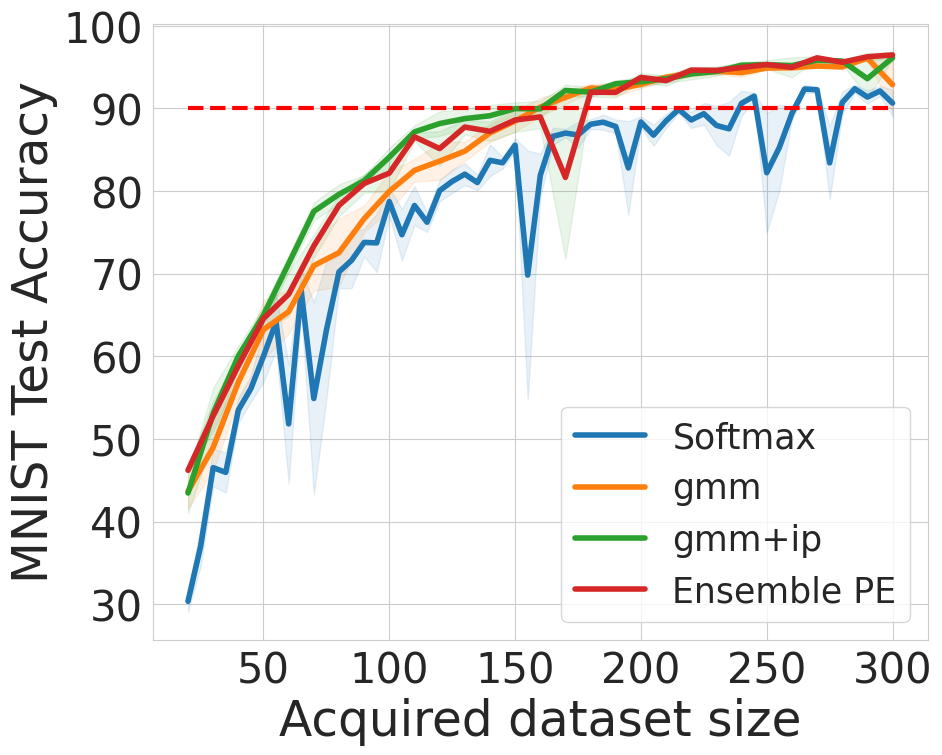
\includegraphics[width=0.75\linewidth]{assets/3-11.png}
    \caption{主动学习任务上对比}
    \label{fig:enter-label}
\end{figure}

\section{本章小结}
结论
